\chapter{Megvalósítás és alkalmazás}
\label{ch:impl}

\section{A meglevő alkalmazások bővítése}
\label{ch:application-improvement}

\subsection {Az asztali alkalmazás bővítése}

A meglevő asztali alkalmazás alkalmas volt a tanítóadatok hatékony előállítására, de utólag nem lehetett visszanézni, hogy adott műholdfelvételhez milyen tanítóadatok tartoznak, illetve azt sem, hogy az adott tanítóadat hol volt mintavételezve. Az alkalmazás eredetileg egy CSV fájlban \cite{rfc4180} tárolta el az összes pixel spektrális értékeit és indexeit, és ezt lehetett használni tanításra. Ennek az volt a hátránya, hogy nehéz volt áttekinteni illetve kiegészíteni az adatokat. Ezért az asztali alkalmazást kiegészítettem ezzel a funkcionalitással, a tanítóadatok előállítása elmentésekor az alkalmazás létrehoz egy külön raszteres réteget is külön minden műholdfelvételhez, melyen látható, hogy mely területek voltak hozzáadva a tanítóadatok közé, így tetszőleges módon előállítható/ellenőrizhető a tanítóhalmaz.

\subsection {A szerveralkalmazás bővítése}

A szerveralkalmazás és webalkalmazás is bővítésre került: a szerveralkalmazás mostmár több modellt is le tud futtatni a letöltött műholdfelvételeken és ezeket külön tárolja. A webalkalmazás mostmár képes letölteni külön ezeket az eredményeket és több hulladékmaszkoló módszer eredményét is meg tudja jeleníteni, ennek köszönhetően ezeket egymással össze lehet könnyen hasonlítani valós tesztadatokon. 

\section{A Tiszta-Tisza alkalmazás}

A Tiszta-Tisza webalkalmazás \todo{melyik link kerüljön ide?} a PET Kupa által használt webalkalmazás, melynek az a célja, hogy egy olyan felületet biztosítson, ahol meglehet tekinteni a jelenleg ismert folyómentén található hulladéklerakókat, illetve akár a regisztrált felhasználók is be tudnak jelenteni ilyet. A PET Kupa megbízta az egyetemet azzal a feladattal, hogy ezt továbfejlessze, és a feladatok közé tartozott az is, hogy a Random Forest modell eredményeit integráljuk ebbe az alkalmazásba. Ezt a feladatot én vállaltam el.

Tekintve arra, hogy a Tiszta-Tisza térképén pontok vannak megjelenítve, a modell által detektált területeket is pontokkal jelöljük. Ehhez egy nagyobb terület közepére helyezünk el egy pontot. Előfordulhat olyan is, hogy a modell olyan képeket klasszifikál, melyek el vannak torzítva (például magas páratartalom miatt). Ilyenkor a false-positive-ok aránya lényegesen megnő. Ennek korrigálására a Tiszta-Tisza alkalmazásban a legutolsó három detektálást (legfeljebb 1 hónap különbséggel) veszem figyelembe és két kép közös metszetével döntöm el, hogy milyen területek kerülnek fel a térképre. A \ref{fig:clean-tisza} ábrán láthatóak a hulladékdetektálás során előállított pontok a térképen, melyeket egy nagyítóval vannak jelölve, melyben van egy felkiáltójel. A Hulladékdetektálás konverzióját a térképen látható pontokká a \ref{ch:intersection} fejezetben részletezem.

\begin{figure}[H]
	\centering
	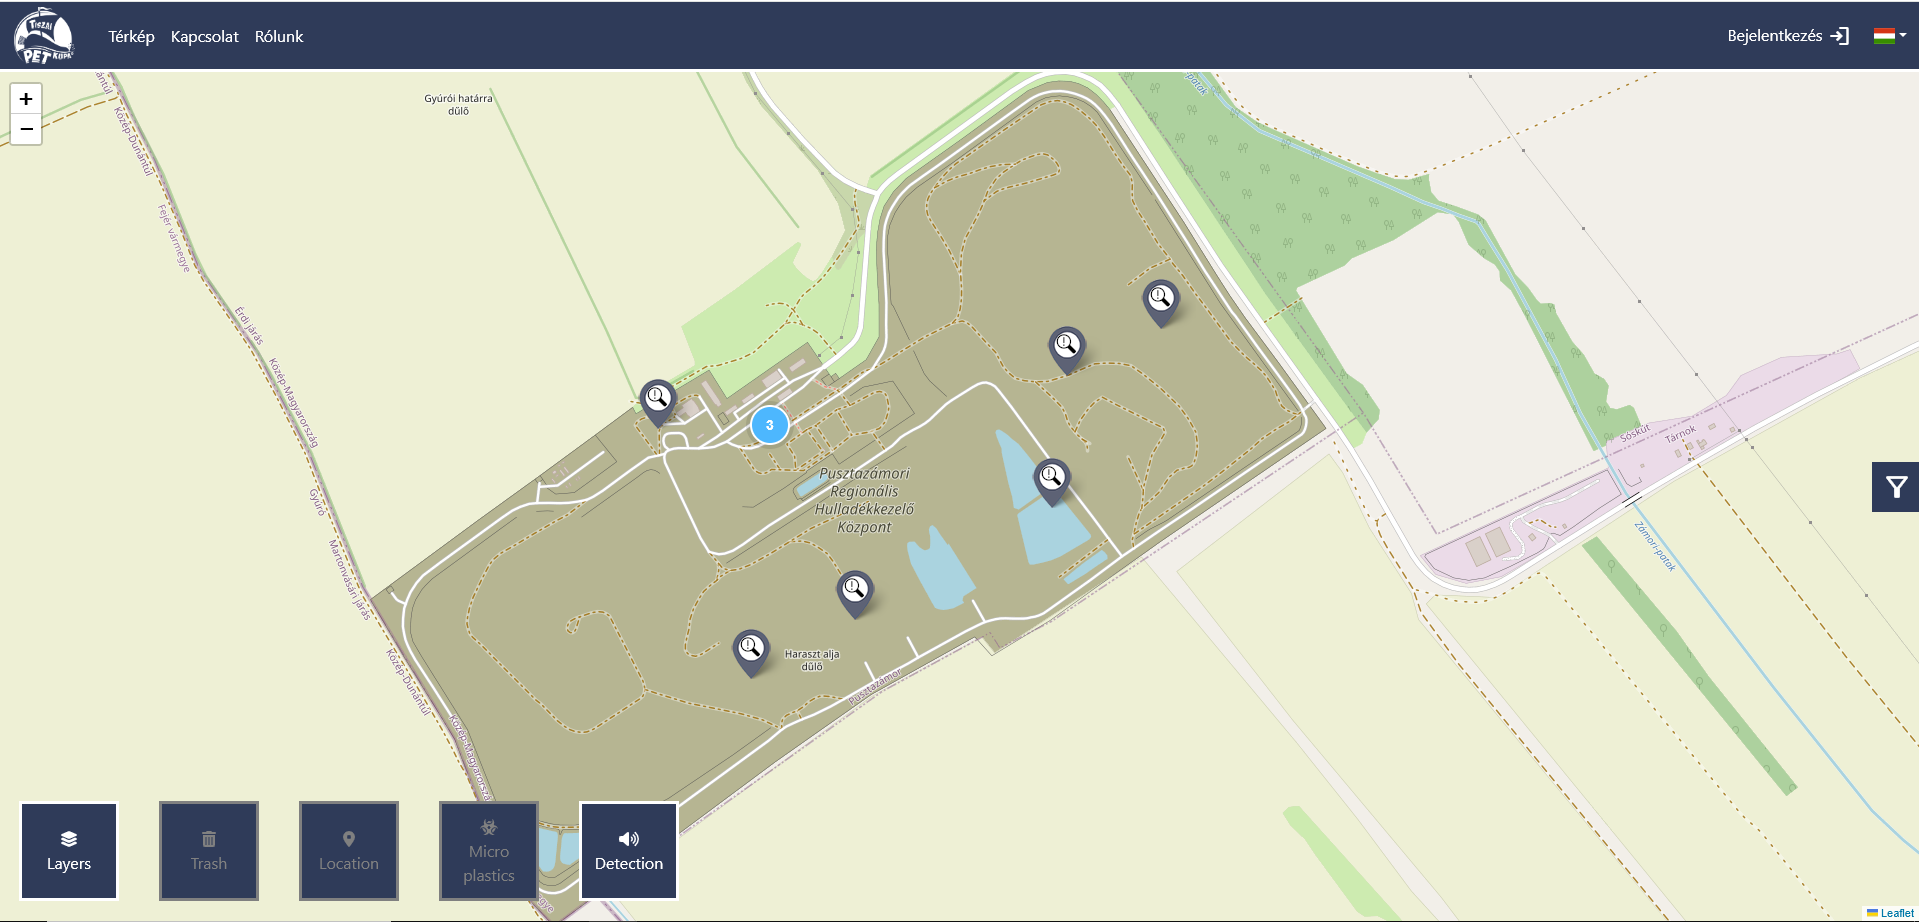
\includegraphics[width=\textwidth,frame]{clean-tisza}
	\caption{A hulladékdetektálás által megjelenített pontok a térképen.}
    \label{fig:clean-tisza}
\end{figure}

\subsection {A képfeldolgozás gyorsítása}
A meglevő képfeldolgozó algoritmuson gyorsítani kellett, hogy elfogadható időn belül tudja feldolgozni a tanítóadatokat, illetve a naponta letöltött műholdfelvételeket a szerveren. Ezt a kutatólabor korábbi cikkjében párhuzamosítással javasolták, de egy egyszálú megoldással lényegesen tudtam gyorsítani a képfeldolgozáson: Ehhez egy nagyon hatékony Python programcsomagot, a Numpy-t \cite{harris2020array} használtam fel, mellyel lényegesen megnöveltem a feldolgozás sebességét: A tanítóadatok feldolgozásakor a régi módszer (\ref{src:old-code} forráskód) 16 felvételt tudott feldolgozni 4 nap és 10 óra alatt, míg az átírt módszer (\ref{src:new-code} forráskód) feldolgozott 85 felvételt 20 perc alatt.

\lstset{caption={A képfeldolgozás régi módszere}, label=src:old-code}
\begin{lstlisting}[language={Python}]
def _calculate_index(numerator: np.ndarray, denominator: np.ndarray) -> np.ndarray:
    """
    Calculating an index based on given numerator and denominator.

    :param numerator: numerator matrix
    :param denominator: denominator matrix
    :return: result matrix, containing the calculated values
    """

    # variables
    rows = numerator.shape[0]
    cols = numerator.shape[1]
    index = np.ndarray(
        shape=numerator.shape,
        dtype="float32",
    )

    # calculate index
    for i in range(rows):
        for j in range(cols):
            if np.isnan(numerator[i, j]) or np.isnan(denominator[i, j]):
                index[i, j] = float("NaN")
            elif denominator[i, j] != 0:
                index[i, j] = numerator[i, j] / denominator[i, j]
            else:
                if numerator[i, j] < 0:
                    index[i, j] = np.nanmin(numerator)
                elif numerator[i, j] > 0:
                    index[i, j] = np.nanmax(numerator)
                else:
                    index[i, j] = float("NaN")

    # return index values
    return index
\end{lstlisting}

\lstset{caption={A képfeldolgozás numpy-al}, label=src:new-code}

\begin{lstlisting}[language={Python}]
def calculate_index(numerator: np.ndarray, denominator: np.ndarray) -> np.ndarray:
    """
    Calculating an index based on given numerator and denominator.
    
    :param numerator: numerator matrix
    :param denominator: denominator matrix
    :return: result matrix, containing the calculated values
    """
    
    # variables
    index = np.ndarray(
        shape=numerator.shape,
        dtype="float32",
    )
    
    numerator_nan_min = np.nanmin(numerator)
    numerator_nan_max = np.nanmax(numerator)
    
    # calculate index
    nan_mask = np.isnan(numerator) | np.isnan(denominator)
    numerator_zero_mask = numerator == 0
    denominator_zero_mask = denominator == 0
    
    invalid_mask = nan_mask | (numerator_zero_mask & denominator_zero_mask)
    valid_mask = np.logical_not(invalid_mask)
    
    valid_denominator_non_zero_mask = valid_mask & np.logical_not(denominator_zero_mask)
    valid_denominator_zero_mask = valid_mask & denominator_zero_mask
    
    numerator_positive_denominator_zero_mask = valid_denominator_zero_mask & (numerator > 0)
    numerator_negative_denominator_zero_mask = valid_denominator_zero_mask & (numerator < 0)
    
    index[invalid_mask] = float("NaN")
    index[numerator_positive_denominator_zero_mask] = numerator_nan_max
    index[numerator_negative_denominator_zero_mask] = numerator_nan_min
    index[valid_denominator_non_zero_mask] = (
        numerator[valid_denominator_non_zero_mask] / denominator[valid_denominator_non_zero_mask]
    )
    
    # return index values
    return index
\end{lstlisting}

\section{Közös metszet}
\label{ch:intersection}

A már meglevő szervertől poligonok formájában, GeoJSON-ben \cite{rfc7946} lehet lekérni az adott napon detektált hulladékos területeket. így érdemes poligonok metszetében kigondolni a többségi szavazást. Jelöljük BUF(P,n)-vel egy multipoligon pufferét, ahol $P \in \mathbb{P}$ egy multipoligon, és n egy egész szám. Ekkor a többségi szavazást három képre a \ref{eq:voting} \todo{hasonló képleteket mások is ismernek fórumokban, de hivatalos forrással nem találkoztam} képlet szerint lehet alkalmazni. Ezután a poligonok egy-egy belső pontját megválasztva megtudjuk jelölni a hulladéklerakókat. A megközelítés szavakra bontva a következő: az összes multipoligon párra vesszük a két multipoligon metszetét, (ahol egy n méretű hibahatár is belefér a metszet számolásba), utána a poligonpárokat rendre összeúniózzuk. A \ref{fig:union-intersection} ábra vizualizálja a képlet lépéseit.

\begin{equation}\label{eq:voting}
    Eredm\acute{e}ny \ multipoligon = \bigcup_{P_1 \in \mathbb{P}} \bigcup_{P_2 \in \mathbb{P}} BUF(BUF(P_1,n) \cap BUF(P_2,n),-n)
\end{equation}

\begin{figure}[H]
	\centering
	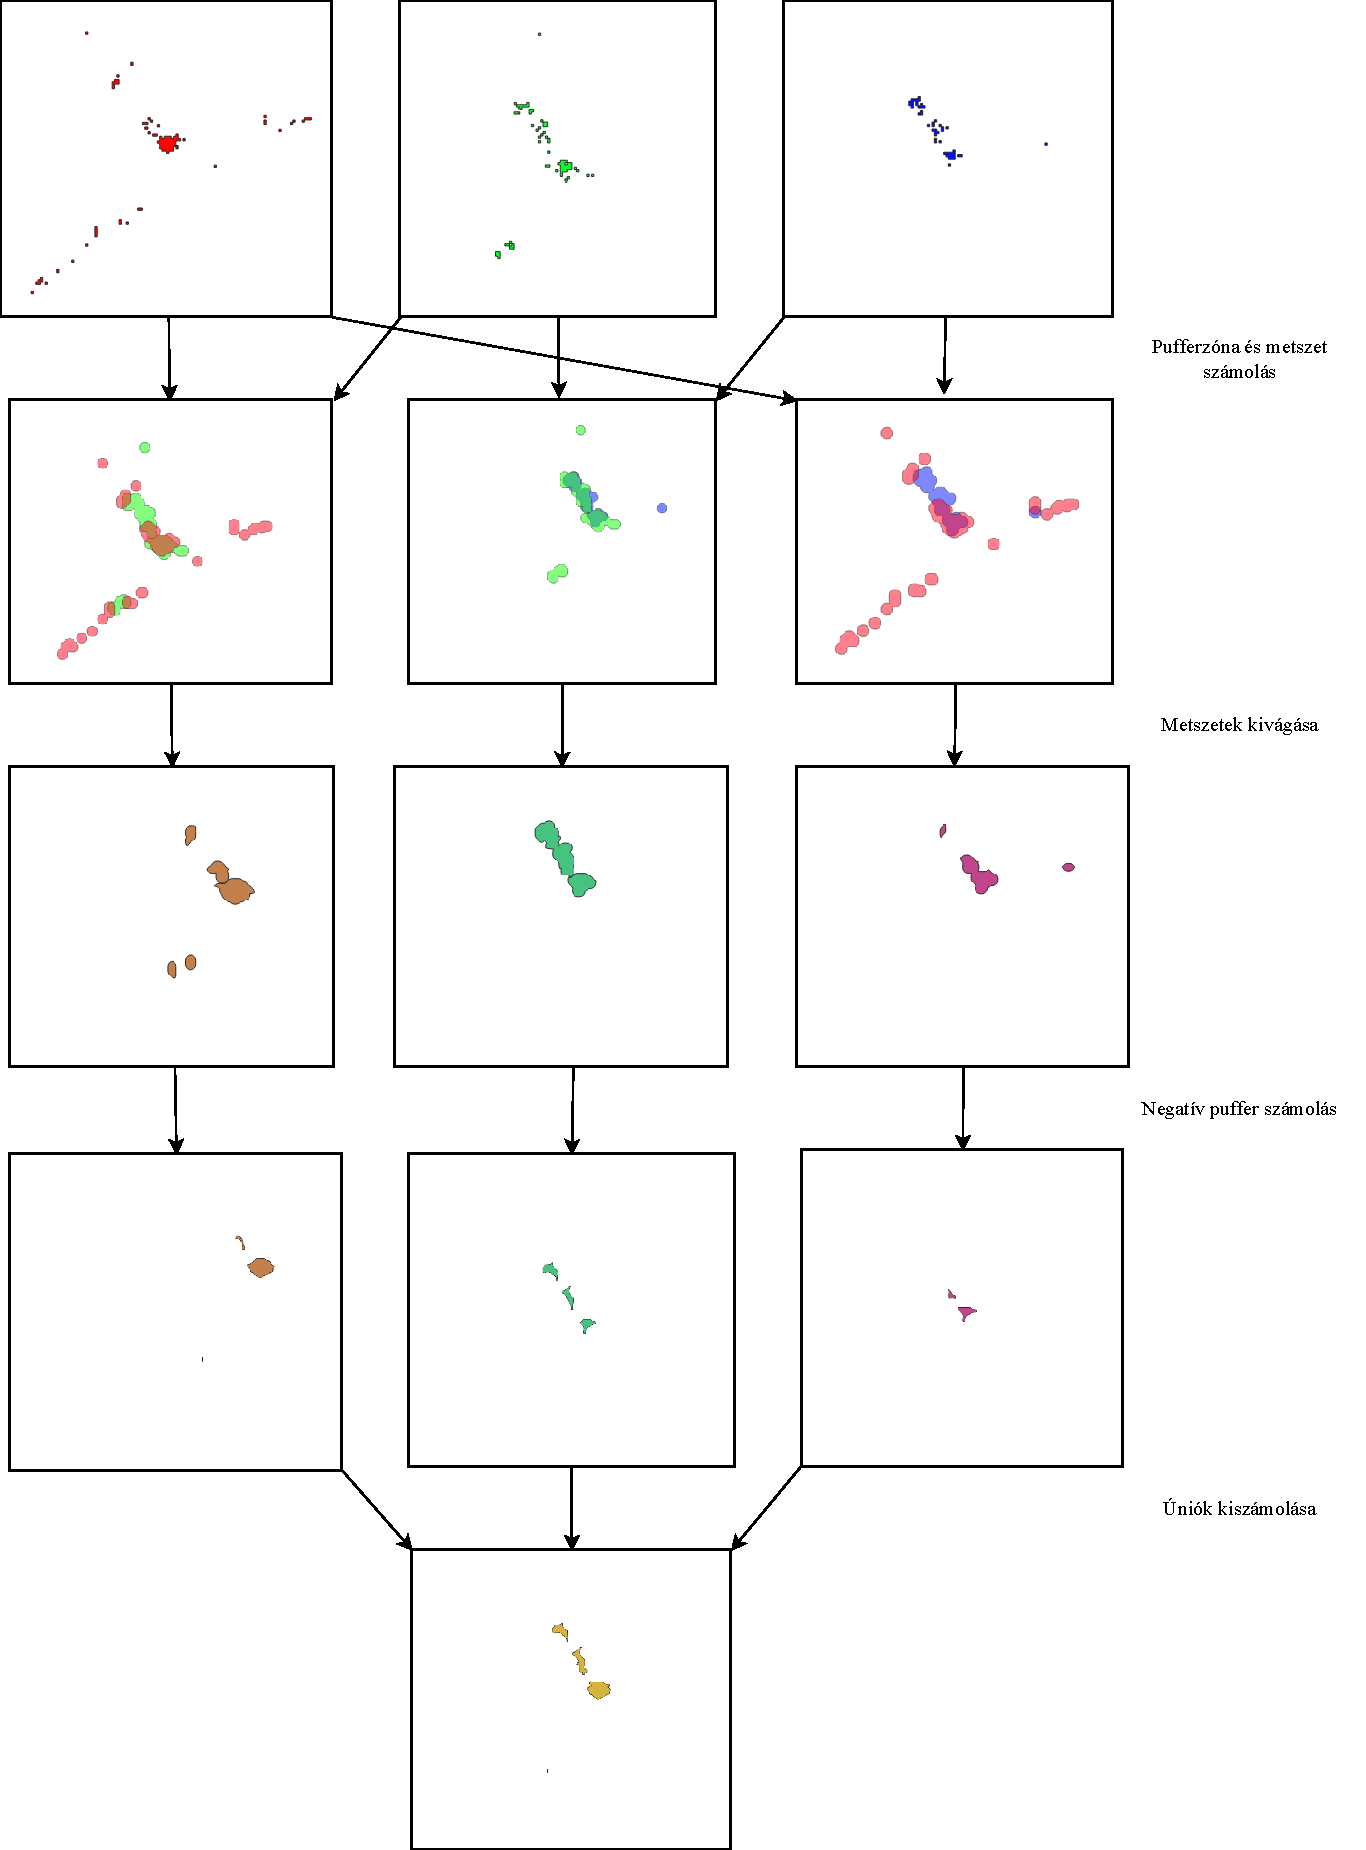
\includegraphics[width=\textwidth,frame]{Waste_markings_flow}
	\caption{A \ref{eq:voting} képlet lépései}
    \label{fig:union-intersection}
\end{figure}